\chapter{Kortste afstanden II}
\begin{itemize}
	\item Het traditioneel algoritme om de kortste afstand tussen twee knopen te bepalen is het algoritme van Dijkstra.
	\item Probleem:
	\begin{itemize}
		\item Dijkstra gebruikt het feit dat indien een pad naar A $\rightarrow$ C bestaat met kost $K_{A, C}$, er geen korter pad A $\rightarrow$ B $\rightarrow$ C kan zijn met kost $K_{A, B} + K_{A, C}$, daarom is het algoritme performant, maar er mogen dus geen negatieve verbindingen zijn. Indien $K_{A, B}$ negatief zou zijn dan klopt Dijkstra niet want dan 

		\begin{align*}
			K_{A, B} + K_{A, C} > K_{A, C}
		\end{align*}
	\end{itemize}
	\item Volgende algoritmen hebben enkel betrekking tot \textbf{gerichte grafen} met mogelijks \textbf{negatieve gewichten}.

\end{itemize}
\section{Kortste afstanden vanuit één knoop}
\subsection{Algoritme van Bellman-Ford}
\begin{itemize}
	\item  Werkt voor negatieve verbindingen.
	\item  Geen globale kennis nodig van heel het netwerk, zoals bij Dijkstra, maar slechts enkel de buren van een bepaalde knoop. Daarom gebruiken routers Bellman-Ford (distance vector protocol).
	\alert  Zal niet stoppen indien er een negatieve lus in de graaf zit, aangezien het pad dan zal blijven dalen tot $-\infty$. 
\end{itemize}

Het algoritme berust op een belangrijke eigenschap: Indien een graaf geen negatieve lussen heeft, zullen de kortste wegen evenmin lussen hebben en hoogstens $n - 1$ verbindingen bevatten. Hieruit kan een recursief verband opgesteld worden tussen de kortste wegen met maximaal $k$ verbindingen en de kortste wegen met maximaal $k - 1$ verbindingen.
$$d_i(k) = \min(d_i(k - 1), \min\limits_{j \in V} (d_j(k - 1) + g_{ji}))$$
met
\begin{itemize}
	\item $d_i(k)$ het gewicht van de kortste weg met maximaal $k$ verbindingen vanuit de startknoop naar knoop $i$,
	\item $g_{ji}$ het gewicht van de verbinding $(j, i)$,
	\item $j \in V$ is elke knoop $j$.
\end{itemize}




Er bestaan \underline{twee goede implementaties}:
\begin{enumerate}
	\item \begin{itemize}
		\item  Niet nodig om in elke iteratie alle verbindingen te onderzoeken. Als een iteratie de voorlopige kortste afstand tot een knoop niet aanpast, is het zinloos om bij de volgende iteratie de verbindingen vanuit die knoop te onderzoeken.
		\item  Plaats enkel de knopen waarvan de afstand door de huidige iteratie gewijzigd werd in een wachtrij.
		\item  Enkel de buren van deze knopen worden in de volgende iteratie getest.
		\item  Elke buur moet, indien hij getest wordt en nog niet in de wachtrij zit, ook in de wachtrij gezet worden.
	\end{itemize}
	\item \begin{itemize}
		\item Gebruik een deque in plaats van een wachtrij.
		\item Als de afstand van een knoop wordt aangepast, en als die knoop reeds vroeger in de deque zat, dant voegt men vooraan toe, anders achteraan.
		\item Kan in bepaalde gevallen zeer inefficiënt uitvallen.
	\end{itemize}

\end{enumerate}

\section{Kortste afstanden tussen alle knopenparen}
\begin{itemize}
	\item Voor dichte grafen $\rightarrow$ Floyd-Warshall (Algoritmen I).
	\item Voor ijle grafen $\rightarrow$ Johnson.
\end{itemize}
\subsection{Het algoritme van Johnson}
\begin{itemize}
	\item Maakt gebruik van Bellman-Ford en Dijkstra.
	\item Omdat we Dijkstra gebruiken, moet elk gewicht positief worden. 
	\begin{enumerate}
		\item Breidt de graaf uit met een nieuwe knoop $s$, die verbindingen van gewicht nul krijgt met elke andere knoop.
		\item Voer Bellman-Ford uit op de nieuwe graaf om vanuit $s$ de kortste afstand $d_i$ te bepalen tot elke originele knoop $i$.
		\item Het nieuwe gewicht $\hat{g}_{ij}$ van een oorspronkelijke verbinding $g_{ij}$ wordt gegeven door: 
		$$\hat{g}_{ij} = g_{ij} + d_i - d_j$$ 
	\end{enumerate}
	\item Het algoritme van Dijkstra kan nu worden toegepast op elke originele knoop, die alle \underline{kortste wegen} zullen vinden. Om de \underline{kortste afstanden} te bepalen moeten de originele gewichten opgeteld worden op deze wegen.
	\item Dit algoritme is $O(n(n + m)\lg n)$ want:
	\begin{itemize}
		\item Graaf uitbreiden is $\Theta(n)$.
		\item Bellman-Ford is $O(nm)$.
		\item De gewichten aanpassen is $\Theta(m)$.
		\item $n$ maal Dijkstra is $O(n(n + m)\lg n)$. Dit is de belangrijkste term, al de andere termen mogen verwaarloosd worden.
	\end{itemize}
\end{itemize}

\section{Transitieve sluiting}
\underline{Sluiting} = algemene methode om één of meerdere verzamelingen op te bouwen. ('als een verzameling deze gegevens bevat, dan moet ze ook de volgende gegevens bevatten').

\begin{itemize}
	\item \textbf{Fixed point}:  Een sluiting wordt fixed point genoemd omdat op een bepaald moment verdere toepassing niets meer verandert, $f(x) = x$.
	\item \textbf{Least fixed point}: De kleinste $x$ zoeken zodat $f(x) = x$ voldaan wordt.
\end{itemize}

\underline{Transitieve sluiting} = 'Als $(a, b)$ en $(b, c)$ aanwezig zijn dan moet ook $(a, c)$ aanwezig zijn.'

\begin{itemize}
	\item Transitieve sluiting van een gerichte graaf is opnieuw een gerichte graaf, maar:
	\begin{itemize}
		\item er wordt een nieuwe verbinding van $i$ naar $j$ toegevoegd indien er een weg bestaat van $i$ naar $j$ in de oorspronkelijke graaf.
	\end{itemize}
	\item \underline{3 algoritmen:}
	\begin{enumerate}
		\item \textbf{Diepte-of breedte-eerst zoeken}: 
				\begin{itemize}
					\item Spoor alle knopen op die vanuit een startknoop bereikbaar zijn en herhaal dit met elke knoop.
					\item Voor ijle grafen $\rightarrow \Theta(n(n + m))$.
					\item Voor dichte grafen $\rightarrow \Theta(n^3)$.
				\end{itemize}
		\item \textbf{Met de componentengraaf}:
				\begin{itemize}
					\item Interessant wanneer men verwacht dat de transitieve sluiting een dichte graaf zal zijn, want dan zijn veel knopen onderling bereikbaar, zodat er een beperkt aantal sterk samenhangende componenten zijn. Die kunnen in $\Theta(n + m)$ bepaald worden.
					\item Maak dan de componentengraaf (kan in $O(n + m))$.
					\item Als nu blijkt dat component $j$ beschikbaar is vanuit component $i$, dan zijn alle knopen van $j$ beruikbaar vanuit knopen van $i$.
				\end{itemize}
		\item \textbf{Het algoritme van Warshall}:
				\begin{itemize}
					\item Maak een reeks opeenvolgende $n \times n$ matrices $T^{(0)},T^{(1)},...,T^{(n)}$ die logische waarden bevatten.
					\item Element $t_{ij}^{(k)}$ duidt aan of er een weg tussen $i$ en $j$ met mogelijke intermediaire knopen $1, 2, ..., k$ bestaat.
					\item Bepalen opeenvolgende matrices:
					$$t_{ij}^{(0)} = 
					\begin{cases}
						\hbox{onwaar} & \hbox{als } i \neq j \hbox{ en } g_{ij} = \infty\\
						\hbox{waar}   & \hbox{als } i = j \hbox{ of } g_{ij} < \infty
					\end{cases}$$
					en
					$$
						t_{ij}^{(k)} = t_{ij}^{(k - 1)} \hbox{ OF } \big(t_{ik}^{(k - 1)} \hbox{ EN } t_{kj}^{(k - 1)}\big) \qquad \hbox{voor } 1 \leq k \leq n
					$$
					\item $T^{(n)}$ is de gezochte burenmatrix.
					\item Alle berekeningen kunnen in dezelfde tabel $T$ gebeuren. Er moet geen plaats voorzien zijn voor andere tabellen.

					\item \textbf{Voorbeeld}
					\begin{figure}[ht]
						\centering
						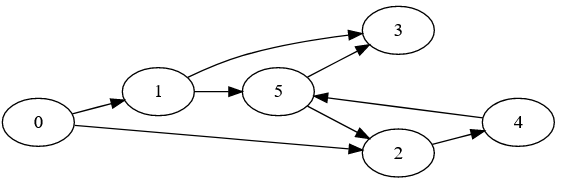
\includegraphics[width=0.5\textwidth]{warshall}
						\caption{Een gerichte graaf met 6 knopen.}
						\label{fig:warshall}
					\end{figure}
					\begin{itemize}
						\item De initieële tabel $T^{(0)}$ is gewoon een kopie van de burenlijst van de graaf.
						$$T^{(0)} = \begin{pmatrix}
							1&1&1&0&0&0\\
							0&1&0&1&0&1\\
							0&0&1&0&1&0\\
							0&0&0&1&0&0\\
							0&0&0&0&1&1\\
							0&0&1&1&0&1
						\end{pmatrix}$$
						\item De tabel $T^{(1)}$ geeft een uitbreiding van $T^{(0)}$, waarbij knoop $1$ een intermediaire knoop mag zijn in een weg naar knopen knopen. Het is logisch dat enkel knopen die $1$ als buur hebben een nieuwe weg kunnen vinden.
						$$T^{(1)} = \begin{pmatrix}
							1&1&1&1&0&1\\
							0&1&0&1&0&1\\
							0&0&1&0&1&0\\
							0&0&0&1&0&0\\
							0&0&0&0&1&1\\
							0&0&1&1&0&1
						\end{pmatrix}$$
						\item De tabel $T^{(2)}$ geeft een uitbreiding van $T^{(1)}$, waarbij knoop $2$ een intermediaire knoop mag zijn in een weg naar twee knopen. Het is logisch dat enkel knopen die $2$ als buur hebben (in de nieuwe matrix $T^{(1)}$) een nieuwe weg kunnen vinden.
						$$T^{(2)} = \begin{pmatrix}
							1&1&1&1&1&1\\
							0&1&0&1&0&1\\
							0&0&1&0&1&0\\
							0&0&0&1&0&0\\
							0&0&0&0&1&1\\
							0&0&1&1&1&1
						\end{pmatrix}$$
						\item Via diezelfde redenering wordt uiteindelijk $T^{(5)}$ bekomen, die de burenmatrix voorstelt van de transitieve sluiting.
						$$T^{(5)} = \begin{pmatrix}
							1&1&1&1&1&1\\
							0&1&1&1&0&1\\
							0&0&1&1&1&1\\
							0&0&0&1&0&0\\
							0&0&1&1&1&1\\
							0&0&1&1&1&1
						\end{pmatrix}$$
						\item Figuur \ref{fig:warshall_solved} toont de transitieve sluiting.
						\begin{figure}[ht]
							\centering
							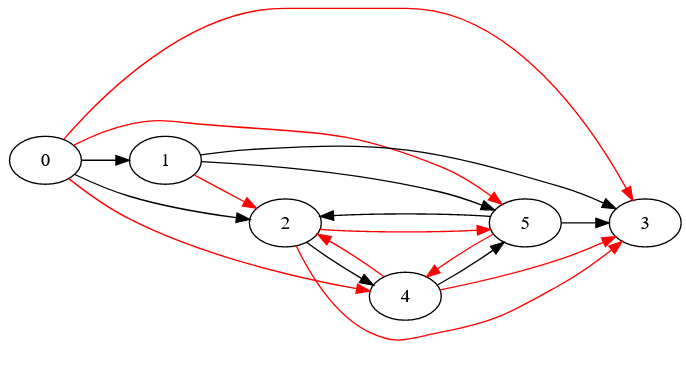
\includegraphics[width=0.75\textwidth]{warshall_solved}
							\caption{De transitieve sluiting van de graaf op figuur \ref{fig:warshall}. De transitieve sluiting bevat dezelfde verbindingen als de graaf (zwarte verbindingen) en ook de nieuwe verbindingen die de transitieve eigenschap vastleggen (rode verbindingen). }
							\label{fig:warshall_solved}
						\end{figure}
					\end{itemize}
				\end{itemize}
				
	\end{enumerate}
\end{itemize}